% !TeX root = Informe_Lab8.tex
% !TeX root = Informe_Lab8.tex
\documentclass[journal]{IEEEtran}
%
\usepackage{instructivo}  
\graphicspath{{./}{./fig/}}
\usepackage{circuitikz}
\usepackage{float}
\usepackage{graphicx}
\usepackage[skip=5pt]{caption}
\usepackage{flafter}
\usepackage{needspace}
\usepackage{csquotes}
\usepackage{upgreek}


\hyphenation{op-tical net-works semi-conduc-tor}

\renewcommand\IEEEkeywordsname{Palabras clave}

\begin{document}
\title{Respuesta en frecuencia de un amplificador BJT}


\author{Juan~P.~Elizondo~Espinoza,~\IEEEmembership{Estudiante,~TEC}
        y~Matías~A.~Camacho~Abarca,~\IEEEmembership{Estudiante,~TEC.}
}


\markboth{TEC.~EL-3215 Laboratorio de Electrónica Analógica, IS~2025}%
{EL3215 Laboratorio de Electrónica Analógica}


\maketitle


\begin{abstract}
    Con este laboratorio se pretendió analizar el comportamiento de los circuitos aplificadores a variaciones de frecuencias extremas, llámese bajas o altas frecuencias. 
    Con lo cual es posible determinar la respuesta en frecuencia de los circuitos y ver si están correctamente construidos para su propósito principal; en caso contrario,
    se prueban algunas maneras de corregir el circuito para que cumpla con su función lo más óptimamente posible.
\end{abstract}

\begin{IEEEkeywords}
Frecuencia, amplificador, ganancia, respuesta, impedancia.
\end{IEEEkeywords}


%%%%%%%%%%%%%%%%%%%%%%%%%%%%%%%%%%%%%%%%%%%%%%%%%%%%%%%%%%%%%%%%%%%%%%%%%%%%%%%%%%%%%%%%%%%%%%
%%%%%%%%%%%%%%%%%%%%%%%%%%%%%%%%%%%%%%%%%%%%%%%%%%%%%%%%%%%%%%%%%%%%%%%%%%%%%%%%%%%%%%%%%%%%%%
\section{Introducción}

\IEEEPARstart{L}a respuesta en frecuencia de un circuito amplificador no es más que el cambio de ganancia o de fase
en un rango de frecuencias aplicadas en la señal de entrada al circuito; dependiendo de la respuesta en frecuencia, 
la salida responderá de una forma u otra~\cite{Floyd}.

Para lograr obtener la respuesta en frecuencia de un circuito amplificador, se le pueden aplicar algunas pruebas
como las realizadas en este laboratorio. Es posible calcular los valores de frecuencia de corte inferior y superior 
para el amplificador, valores que se ven afectados por la capacitancias de acople o bypass en caso de trabajar con bajas
frecuencias, o bien, por las capactiancias presentes entre las terminales del transistor las cuales se vuelven relevantes 
cuando el circuito opera a altas frecuencias~\cite{Floyd}.

En el caso de los transistores BJT (utilizados en este experimento), las capacitancias parásitas se generan por las 
juntas PN que componen al transistor, por lo que sus efectos están presentes "naturalmente". Dependiendo de dónde se investigue, 
las capacitancias pueden recibir nombres diferentes, pero entre los más utilizados están $C_{CS}$ para la junta del
colector y el substrato, $C_{\pi}$ para la junta de la base y el emisor, y $C_{\mu}$ para la unión entre el colector y la base~\cite{Razavi}.

Experimentalmente se puede colocar el circuito a operar en ambos escenarios y recopilar sus frecuencias de corte; para con ello, graficar
el comportamiento de la ganancia según el rango de frecuencias y validar el funcionamiento del amplificador. Tal es el caso de las
pruebas experimentales aplicadas en este laboratorio. 

%%%%%%%%%%%%%%%%%%%%%%%%%%%%%%%%%%%%%%%%%%%%%%%%%%%%%%%%%%%%%%%%%%%%%%%%%%%%%%%%%%%%%%%%%%%%%%
%%%%%%%%%%%%%%%%%%%%%%%%%%%%%%%%%%%%%%%%%%%%%%%%%%%%%%%%%%%%%%%%%%%%%%%%%%%%%%%%%%%%%%%%%%%%%%
\section{Cirtuitos para las mediciones}
Se presenta a continuación los circuitos construidos para la elaboración de este laboratorio. 
Se montaron 2 circuitos de tal manera que el circuito 1 sirvió para estudiar la respuesta en bajas frecuencias y el circuito 2 para estudiar la respuesta en altas frecuencias. 
Los transistores utilizados fueron BJTs 2N3904.
Se midieron los parámetros de polarización en corriente directa y parámetros en corriente alterna.


\subsection{Circuitos de Medición}

\begin{figure}[H]
        \centering
        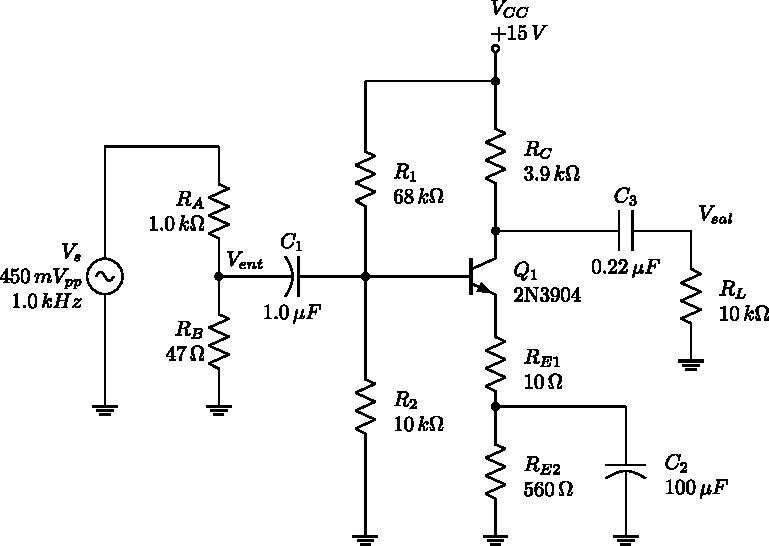
\includegraphics[width=3.4in]{CIRCUITO1.pdf}
        \caption{Circuito 1}
        \label{fig:SignalExperimental_024}
\end{figure}

\begin{figure}[H]
        \centering
        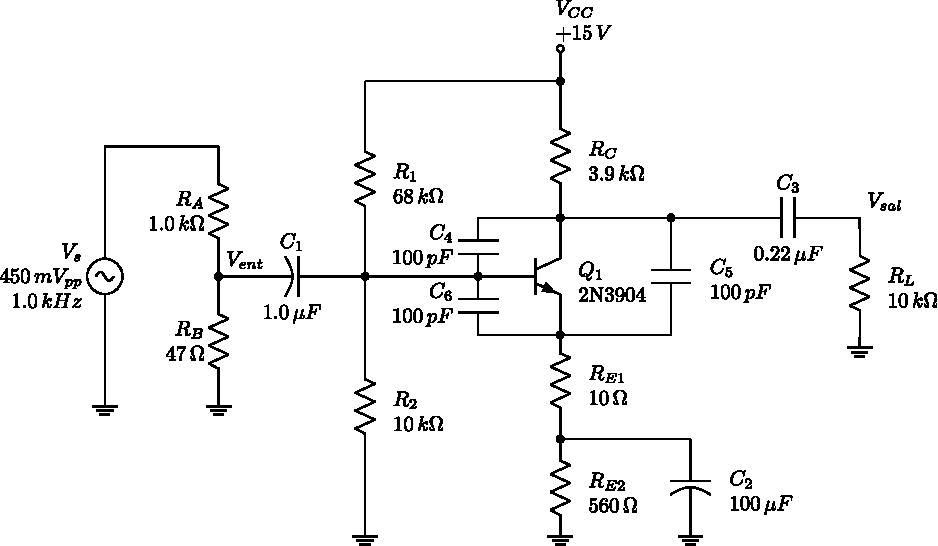
\includegraphics[width=3.4in]{CIRCUITO2.pdf}
        \caption{Circuito 2}
        \label{fig:SignalExperimental_044}
\end{figure}

\vspace{1cm}


\subsection{Resultados}


\begin{table}[H]
        \centering
        \renewcommand{\arraystretch}{1.5}
        \caption{Valores de resistencias utilizadas en los circuitos 1 y 2}
        \begin{tabular}{ >{\centering\arraybackslash}m{2.5cm} >{\centering\arraybackslash}m{2.5cm} >{\centering\arraybackslash}m{2.5cm} }
                \hline
            \centering
            Componente & Valor requerido & Valor medido\\ 
            \hline
            \centering
            $R_A$ ($\mathrm{k}\Omega$) & $1$  & $1.000~58$  \\ 
            $R_B$ ($\Omega$) & $47$  & $49.907~6$  \\
            $R_C$ ($\mathrm{k}\Omega$) & $3.9$  & $3.855~47$  \\
            $R_1$ ($\mathrm{k}\Omega$) & $68$  & $67.771~6$ \\
            $R_2$ ($\mathrm{k}\Omega$) & $10$  & $9.925~77$ \\
            $R_L$ ($\mathrm{k}\Omega$) & $10$  & $9.937~73$ \\
            $R_{E1}$ ($\Omega$) & $10$  & $10.024~8$ \\
            $R_{E2}$ ($\Omega$) & $560$  & $555.329$ \\
            \hline
        \end{tabular}
        \label{tabla1}
    \end{table}
    
\begin{table}[H]
        \centering
        \renewcommand{\arraystretch}{1.5}
        \caption{Valores de capacitores utilizados en el circuito 1}
        \begin{tabular}{ >{\centering\arraybackslash}m{2.5cm} >{\centering\arraybackslash}m{2.5cm} >{\centering\arraybackslash}m{2.5cm} }
                \hline
            Componente & Valor requerido ($\upmu\mathrm{F}$) & Valor medido ($\upmu\mathrm{F}$)\\ 
            \hline
            \centering
            $C_1$ & $1$  & $1.038~3$  \\ 
            $C_2$ & $100$  & $94$ \\
            $C_3$ & $0.22$  & $0.258~6$ \\
            \hline
        \end{tabular}
        \label{tabla2}
    \end{table}    

\begin{table}[H]
        \centering
        \renewcommand{\arraystretch}{1.5}
        \caption{Valores de capacitores utilizados en el circuito 2}
        \begin{tabular}{ >{\centering\arraybackslash}m{2.5cm} >{\centering\arraybackslash}m{2.5cm} >{\centering\arraybackslash}m{2.5cm} }
                \hline
            Componente & Valor requerido & Valor medido\\ 
            \hline
            \centering
            $C_1$ ($\upmu\mathrm{F}$) & $1$  & $1.038~3$  \\ 
            $C_2$ ($\upmu\mathrm{F}$) & $100$  & $94$ \\
            $C_3$ ($\upmu\mathrm{F}$) & $0.22$  & $0.258~6$ \\
            $C_4$ ($\mathrm{p}$) & $100$ & $98.3$ \\
            $C_5$ ($\mathrm{p}$) & $100$ & $104.5$ \\
            $C_6$ ($\mathrm{p}$) & $100$ & $90.3$ \\
            \hline
        \end{tabular}
        \label{tabla3}
    \end{table}   

Para realizar el cálculo de las frecuencias críticas de corte inferior del circuito 1, se procedió a aislar los capacitores de los efectos de los otros capacitores. Por ejemplo, se colocó un capacitor de $1000~\upmu\mathrm{F}$ en paralelo de C\textsubscript{2} y otro sobre C\textsubscript{3}; esto causó que la respuesta en frecuencia de estos capacitores tenga muy poco efecto sobre la salida del amplificador.
La señal de salida en banda media se ajustó a alrededor de $10~\mathrm{kHz}$ y se ajustó la
señal para ser observada hasta una caída en la ganancia de $3~\mathrm{dB}$. La frecuencia a la que se dio esa reducción representó la frecuencia crítica inferior debido al capacitor C\textsubscript{1}. El mismo procedimiento
se realizó para C\textsubscript{2} y C\textsubscript{3}.

\begin{table}[H]
        \centering
        \renewcommand{\arraystretch}{1.5}
        \caption{Frecuencias críticas de corte inferior, circuito 1}
        \begin{tabular}{ >{\centering\arraybackslash}m{2.5cm} >{\centering\arraybackslash}m{2.5cm} >{\centering\arraybackslash}m{2.5cm} }
                \hline
            Capacitor & Valor requerido ($\mathrm{Hz}$) & Valor medido ($\mathrm{Hz}$)\\ 
            \hline
            \centering
            $C_1$ & $51.303~8$  & $54.118$  \\ 
            $C_2$ & $69.812~4$  & $68.942$ \\
            $C_3$ & $52.045~4$  & $45.983$ \\
            $\mathrm{General}$ & $173.161~6$  & $125.83$ \\
            \hline
        \end{tabular}
        \label{tabla4}
    \end{table}    

También se calculó el valor de la frecuencia crítica inferior de C\textsubscript{2} si el valor de C\textsubscript{2} fuera modificado a aproximadamente $35.5~\upmu\mathrm{F}$ para conseguir una frecuencia de corte
general de $300~\mathrm{Hz}$.

\begin{table}[H]
        \centering
        \renewcommand{\arraystretch}{1.5}
        \caption{Frecuencias críticas de corte inferior de $C_2$, bsucando que la frecuencia crítica general inferior sea de $\mathrm{300~Hz}$}
        \begin{tabular}{ >{\centering\arraybackslash}m{2.5cm} >{\centering\arraybackslash}m{2.5cm} >{\centering\arraybackslash}m{2.5cm} }
                \hline
            Valor calculado de $C_2$ & Valor teórico ($\mathrm{Hz}$) & Valor medido ($\mathrm{Hz}$)\\ 
            \hline
            \centering
            $C_2$ & $196.650~8$  & $209.899$  \\ 
            \hline
        \end{tabular}
        \label{tabla11}
    \end{table}  
Es importante que debido al bajo valor de V\textsubscript{ent}, se estimó este como $10~mV$ para ambos circuitos. 
\begin{table}[H]
        \renewcommand{\arraystretch}{1.5}
        \caption{Mediciones del circuito 1}
        \centering
        \begin{tabular}{ >{\centering\arraybackslash}m{2.5cm} >{\centering\arraybackslash}m{2.5cm} >{\centering\arraybackslash}m{2.5cm} }
                \hline
            Parámetro & Valor teórico & Valor medido\\ 
            \hline
            $V_B$ ($\mathrm{V}$) & $1.77$  & $1.816~82$  \\ 
            $V_E$ ($\mathrm{V}$) & $1.09$  & $1.157~29$  \\
            $V_C$ ($\mathrm{V}$) & $7.59$  & $7.164~76$  \\
            $V_{CE}$ ($\mathrm{V}$) & $6.50$  & $6.007~47$  \\
            $I_E$ ($\mathrm{mA}$) & $1.92$  & $2.047$ \\ 
            $|A_v|$  & $109.443$ & $115.5$  \\
            $V_{sal}$ & $1.057$  & $1.155$ \\
            \hline
        \end{tabular}
        \label{tabla5}
    \end{table}

\begin{figure}[H]
        \centering
        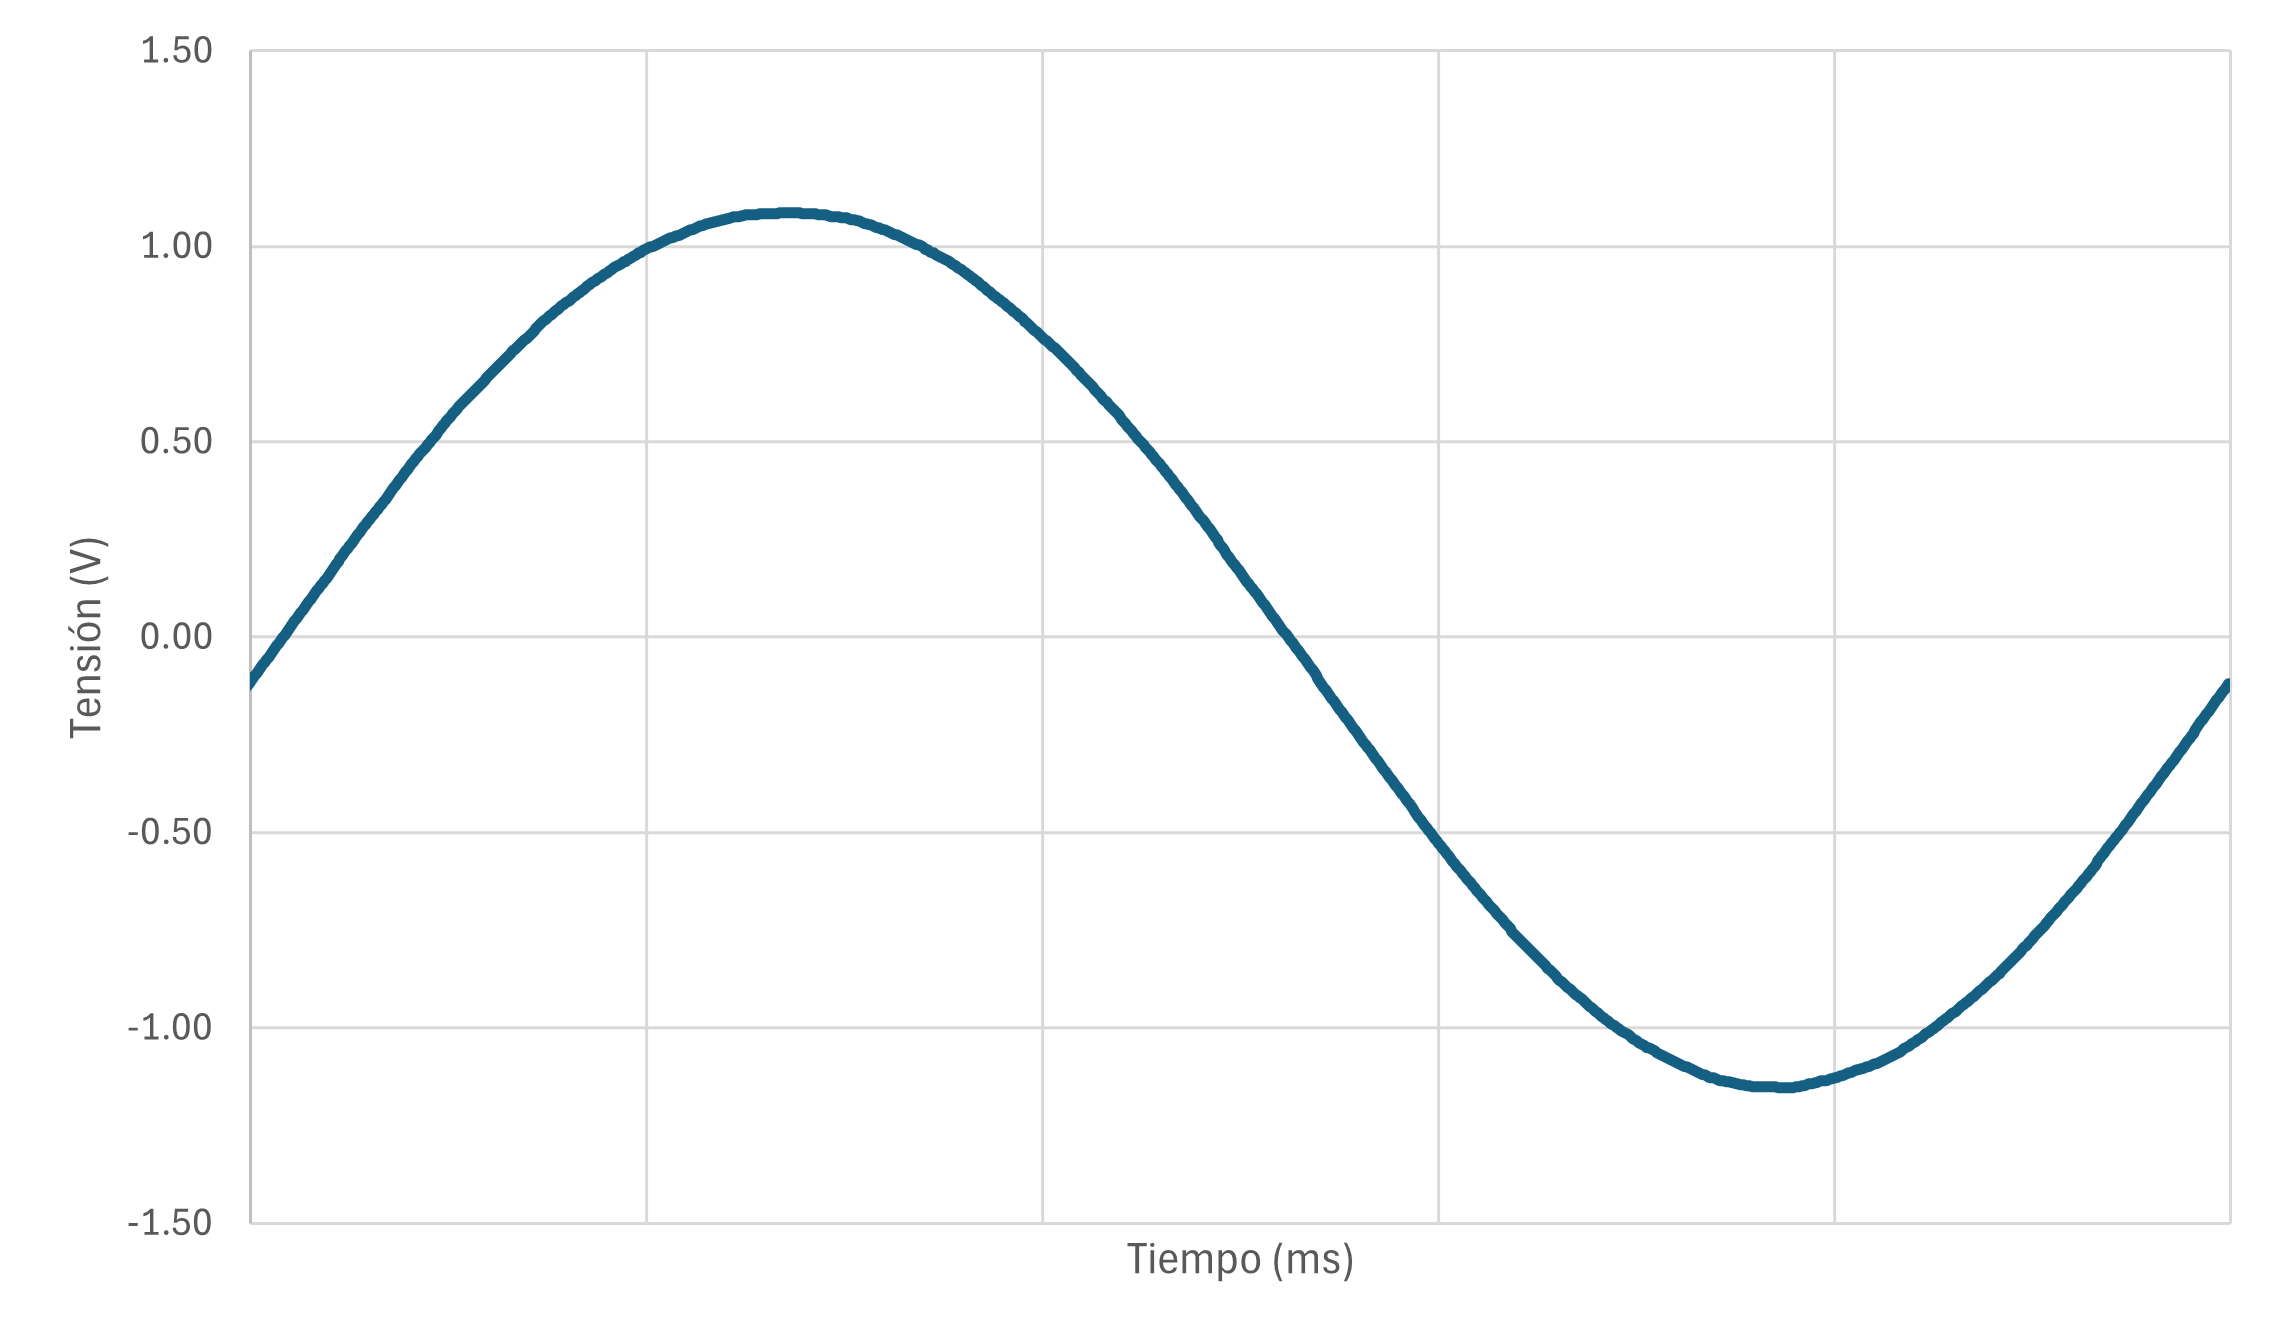
\includegraphics[width=3.4in]{OutC1.png}
        \caption{$V_{sal}$ obtenido experimentalmente en el circuito 1 durante un periodo}
        \label{fig:SignalExperimental_0222}
\end{figure}
    
\begin{table}[H]
        \renewcommand{\arraystretch}{1.5}
        \caption{Mediciones del circuito 2}
        \centering
        \begin{tabular}{ >{\centering\arraybackslash}m{2.5cm} >{\centering\arraybackslash}m{2.5cm} >{\centering\arraybackslash}m{2.5cm} }
                \hline
            Parámetro & Valor teórico & Valor medido\\ 
            \hline
            $V_B$ ($\mathrm{V}$) & $1.811~16$  & $1.806~24$  \\ 
            $V_E$ ($\mathrm{V}$) & $1.129~35$  & $1.156~78$  \\
            $V_C$ ($\mathrm{V}$) & $7.322~96$  & $7.392~27$  \\
            $V_{CE}$ ($\mathrm{V}$) & $6.193~61$  & $6.235~49$  \\
            $I_E$ ($\mathrm{mA}$) & $1.981~31$  & $2.046$ \\ 
            $|A_v|$  & $111.544~9$ & $113.5$  \\
            $V_{sal}$ & $1.175~07$  & $1.135$ \\
            \hline
        \end{tabular}
        \label{tabla6}
    \end{table}

\begin{figure}[H]
        \centering
        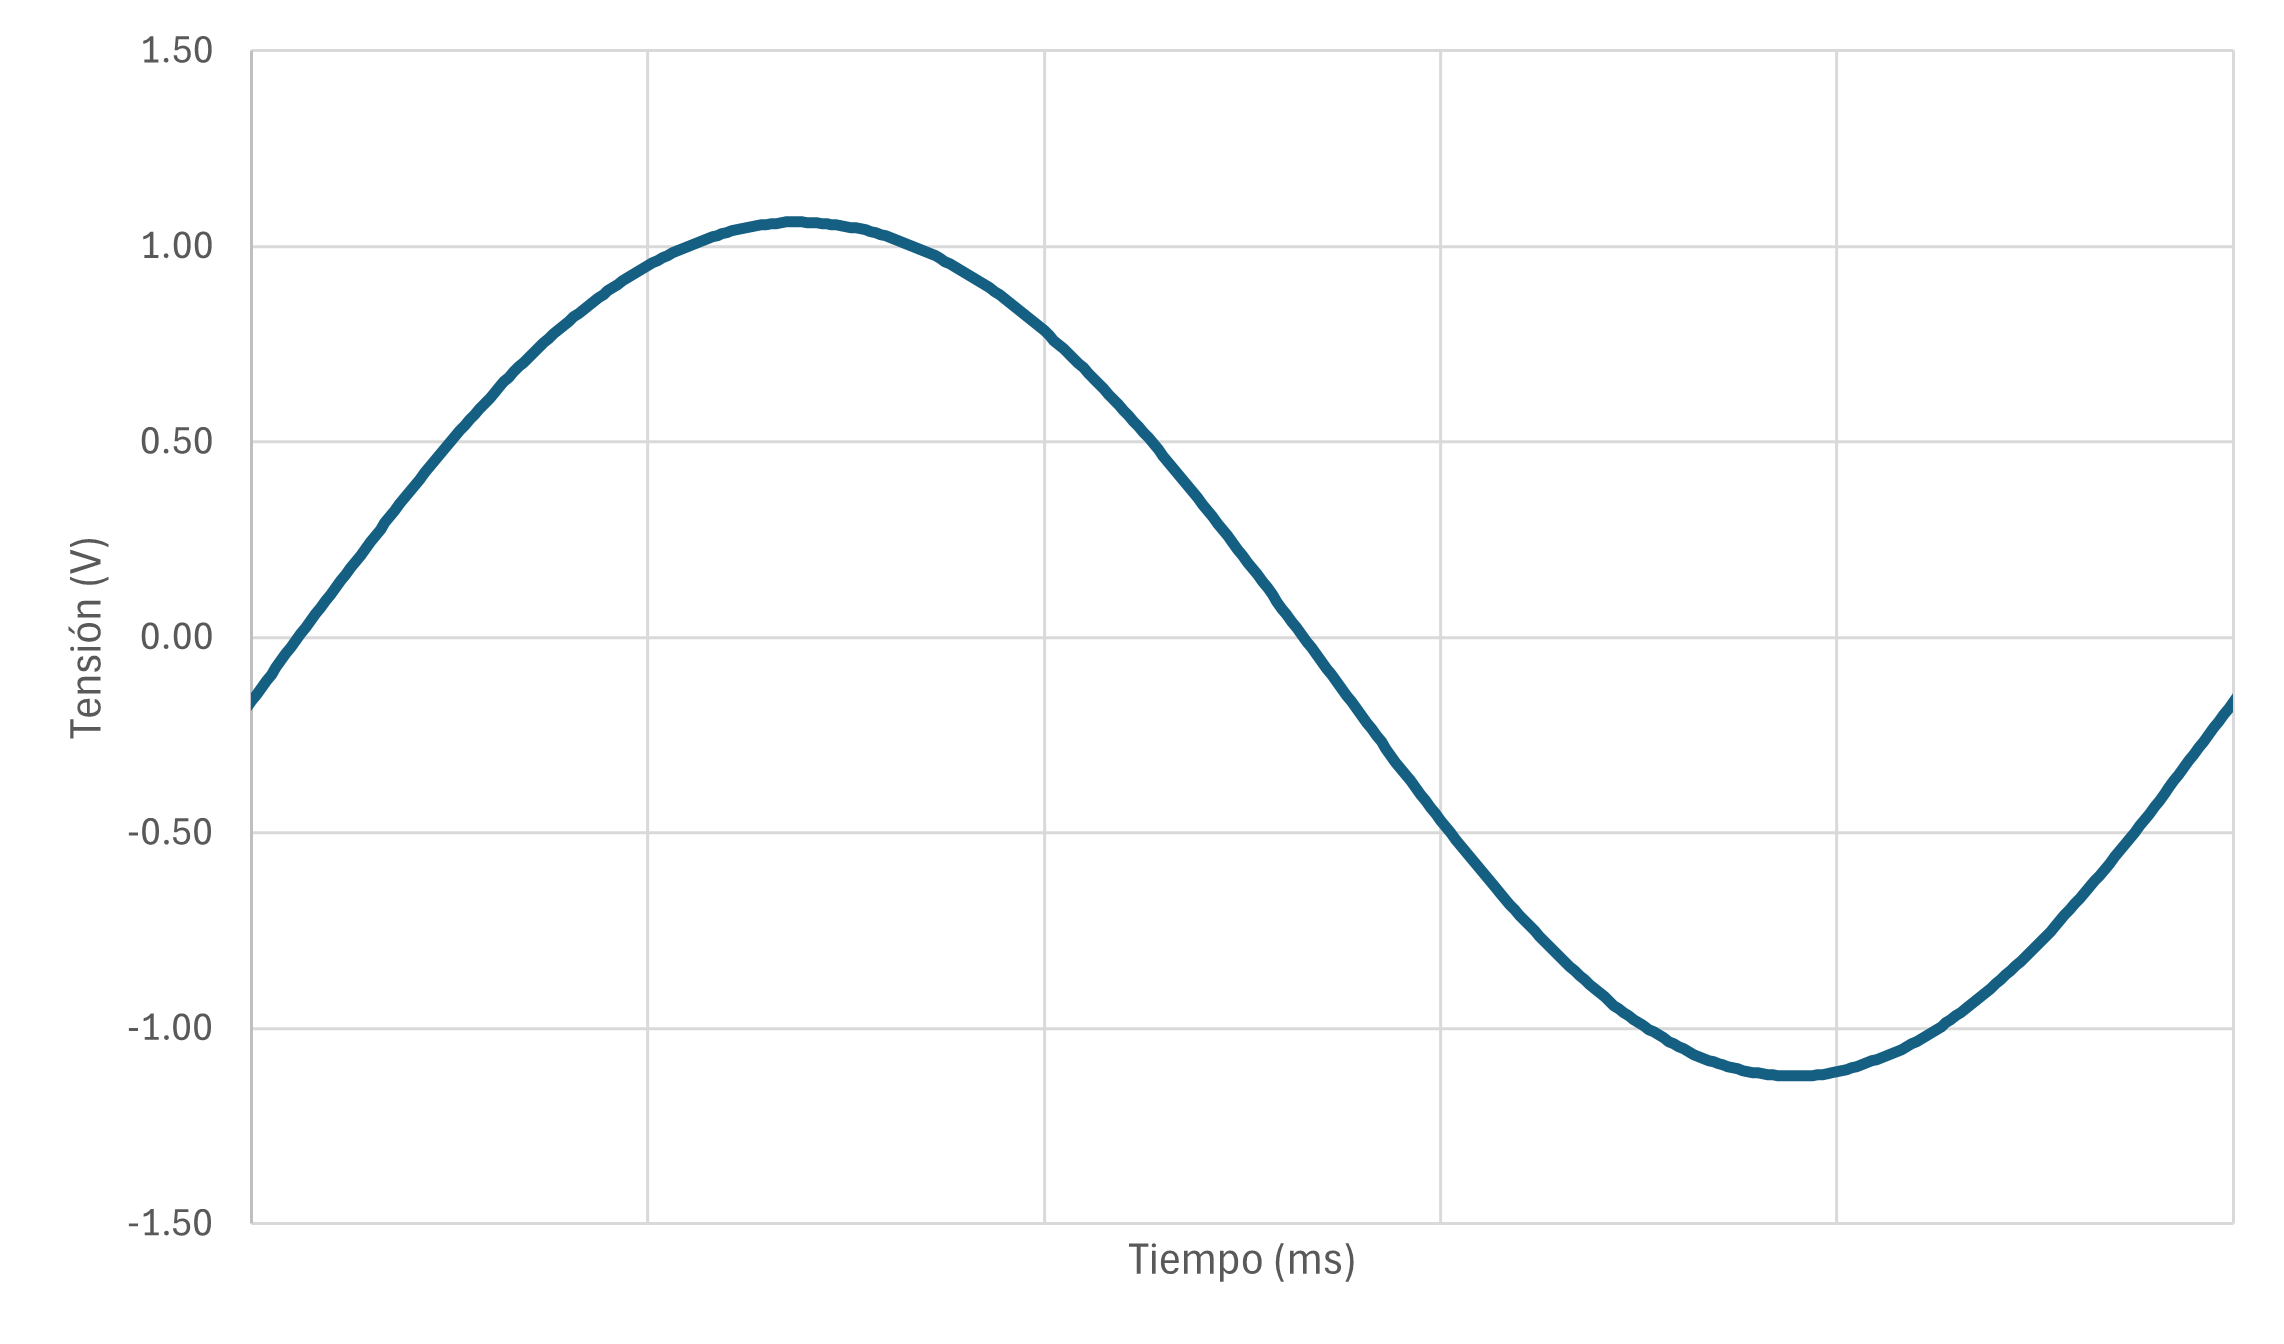
\includegraphics[width=3.4in]{OutC2.png}
        \caption{$V_{sal}$ obtenido experimentalmente en el circuito 2 durante un periodo}
        \label{fig:SignalExperimental_02}
\end{figure}

Para el cálculo de la frecuencia crítica superior general, se modificó la frecuencia de la fuente hasta observar una caida de $3~\mathrm{dB}$.

\begin{table}[H]
        \centering
        \renewcommand{\arraystretch}{1.5}
        \caption{Frecuencias críticas superiores, circuito 2}
        \begin{tabular}{ >{\centering\arraybackslash}m{2.5cm} >{\centering\arraybackslash}m{2.5cm} >{\centering\arraybackslash}m{2.5cm} }
                \hline
            Frecuencia & Valor teórico ($\mathrm{kHz}$) & Valor experimental ($\mathrm{kHz}$)\\ 
            \hline
            \centering
            $f_{c(ent)}$ & $298.853$  & $296.716$  \\
            $f_{c(sal)}$ & $282.357$  & $281.321$  \\
            $f_{cu}$ & $166.331$  & $165.80$  \\ 
            \hline
        \end{tabular}
        \label{tabla7}
    \end{table}   

\subsection{Análisis de Resultados}
En este laboratorio, es de esperar que los resultados experimentales de las mediciones de frecuencia, den algo alejados
a los valores teóricos calculados, ya que se trata de parámetros sensibles a muchos factores que pueden alterar
su resultado. 

En términos generales, para el circuito de análisis a bajas frecuencias. Las frecuencias de corte correspondientes para cada uno
de los capactirores ($C_1$, $C_2$ y $C_3$) presentaron valores bastante cercanos a lo esperado, con una diferencia de al menos $1.247\%$ 
y de un $11.648\%$ en el peor de los casos. La frecuencia de corte inferior, se ubicó en un valor que tal como se esperaba, es menor 
a la aproximación realizada al sumar los tres valores teóricos de frecuencias críticas independientes, ubicándose en los $125.83$ $\mathrm{Hz}$. 

Para el circuito analizado en altas frecuencias, se tiene la frecuencia de corte superior la cual presenta una diferencia del $0.319\%$ 
respecto a lo esperado de forma teórica, lo cual es bastante bueno considerando lo expuesto al principio de esta sección. 


\section{Conclusiones}
Se logró calcular y medir satisfactoriamente la frecuencia crítica inferior para cada uno de los capacitores del primer circuito, 
arrojando resultados ceranos a lo esperado; además, fue posible comprobar que la frecuencia crítica general inferior es menor a la 
aproximación realizada de manera teórica, con un valor de $125.83$ $\mathrm{Hz}$.
En cuanto al segundo circuito, se logró calcular y medir las frecuencias críticas superiores, obteniendo valores con muy poco porcentaje de error, así como una frecuencia crítica general superior menor que la frecuencia crítica superior de entrada y que la frecuencia crítica superior de salida, comportamiento que era esperado.
\appendices

\section{}

\begin{IEEEbiographynophoto}{Matías A. Camacho Abarca}
        Estudiante del Instituto Tecnológico de Costa Rica en la carrerra de ingeniería en electrónica desde
        2023. Beneficiario de beca de excelencia académica por el Instituto Tecnológico de
        Costa Rica desde 2023. Como estudiante, sus
        intereses incluyen investigación y desarrollo.
        Correo electrónico: jeacamacho@estudiantec.cr
\end{IEEEbiographynophoto}

\begin{IEEEbiographynophoto}{Juan P. Elizondo Espinoza}
        Oriundo de Pérez Zeledón. Realizó sus estudios de secundaria en el SNCCCR, sede UNA Región Brunca, y actualmente cursa la carrera de Ingeniería Electrónica en el Instituto Tecnológico de Costa Rica (TEC). 
        
        Anteriormente, fue estudiante de la Universidad de Costa Rica (UCR) durante el año 2022 y participó en programas de estudio en matemática en la Universidad Nacional (UNA) durante los años 2020 y 2021. 
        
        Cuenta con preparación y/o experiencia en áreas como:
        \begin{itemize}
            \item Arquitectura básica de redes, certificado por CISCO CCNA V7 (ITN), (2021).
            \item Principios de ciberseguridad, certificado por CISCO Systems, (2022).
            \item Programa de tutorías estudiantiles, Tecnológico de Costa Rica, (2024).
        \end{itemize}
        
        Correo: juelizondo@estudiantec.cr
\end{IEEEbiographynophoto}

%%\bibliographystyle{IEEEtran}
%%\bibliography{literatura}

\begin{thebibliography}{11}
    \bibitem{Floyd}
    Thomas L. Floyd, \emph{Dispositivos Electrónicos}, 8ª edición, Pearson, 2008.
    \bibitem{Razavi}
    Behzad Razavi, \emph{Fundamentals of Microelectronics}, 2nd edition, Wiley, 2013.

\end{thebibliography}

\end{document}